\def\mytitle{PYTHON PROGRAMMING ON MATRICES}
\def\myauthor{Revathi pamujula}
\def\contact{revathipamujula111@gmail.com}
\def\mymodule{Future Wireless Communication (FWC)}


\documentclass[10pt, a4paper]{article}
\usepackage[a4paper,outer=1.5cm,inner=1.5cm,top=1.75cm,bottom=1.5cm]{geometry}

\twocolumn
\usepackage{graphicx}
%\usepackage{karnaugh-map}
\usepackage{tabularx}
\usepackage{hyperref}
\usepackage[utf8]{inputenc}
\usepackage{amsmath}
%\usepackage{physics}
\usepackage{amssymb}
\usepackage{watermark}
\renewcommand*\familydefault{\sfdefault}
\usepackage{lipsum}
\usepackage{xcolor}
\usepackage{listings}
\let\vec\mathbf
\lstset{
frame=single, 
breaklines=true,
columns=fullflexible
}
\begin{document}
\title{\mytitle}
\author{\myauthor\hspace{1em}\\\contact\\FWC220\hspace{6.5em}IITH\hspace{0.5em}\mymodule\hspace{6em}Matrix:Circle}

%\{ Wireless Communication (FWC)}
\date{}
\maketitle


  \section{Problem}
If the two circles $$ (x- 1)^2+(y-3)^2=r^2 $$ and\\
$$x^2+y^2-8x+2y+8=0$$ intersect in two distinct points, then 
\section{Solution}
\textbf{Given that:}
The circle equation is\\
\begin{center}
%\boldmath
$$\vec{x}^{T}V\vec{x}+2\vec{u}^{T}\vec{x}+f=0$$\\
$r=\sqrt{\left \| \vec{u} \right \|^{2}-f}$
%\unboldmath
\end{center}
Comparing the given equations 1 and 2 with the circle equation to find the centre and radius\\
\textbf{eq(1) can be expressed as}\\
\begin{center}
%\boldmath
$\vec{x}^{T}$$\begin{pmatrix}
1 & 0\\ 
 0 & 1
\end{pmatrix}\vec{x}+2\begin{pmatrix}
-1 & -3
\end{pmatrix}\vec{x}+10=r^{2}$
%\unboldmath
\end{center}
centre and radius are\\

\begin{center}
%\boldmath
$\vec{c}=\vec{-u}$

$\vec{c}=\begin{pmatrix}
1\\ 
3
\end{pmatrix} $
$r_{1}=r$
%\unboldmath
\end{center} 
\textbf{eq(2) can be expressed as}\\
\begin{center}
%\boldmath
$\vec{x}^{T}$$\begin{pmatrix}
1 & 0\\ 
 0 & 1
\end{pmatrix}\vec{x}+2\begin{pmatrix}
-4 & 1
\end{pmatrix}\vec{x}+8=0$
%\unboldmath
\end{center}
centre  and radius are\\

\begin{center}
%\boldmath
$\vec{c} = \vec{-u}$\\
$$\vec{c}=\begin{pmatrix}
4\\ 
-1
\end{pmatrix} $$
$r_{2}=3$
%\unboldmath
\end{center} 
Distance between two points (1,3)=$c_{1}$ and (4,-1)=$c_{2}$
\begin{center}
%\boldmath
$$\left \| \vec{c}_{1}-\vec{c}_{2} \right\|=\sqrt{ (\vec{c}_{1}-\vec{c}_{2})^{T}(\vec{c}_{1}-\vec{c}_{2})}=5$$
%\unboldmath
\end{center} 
Two circles intersect in two distinct point then 
\begin{center}
%\boldmath
$r_{1}-r_{2}<$$\left \| \vec{c}_{1}-\vec{c}_{2} \right\|<r_{1}+r_{2}$\\
$r-3<5<r+3$\\
$2<r<8$
%\unboldmath
\end{center} 
\begin{figure}[h!]
  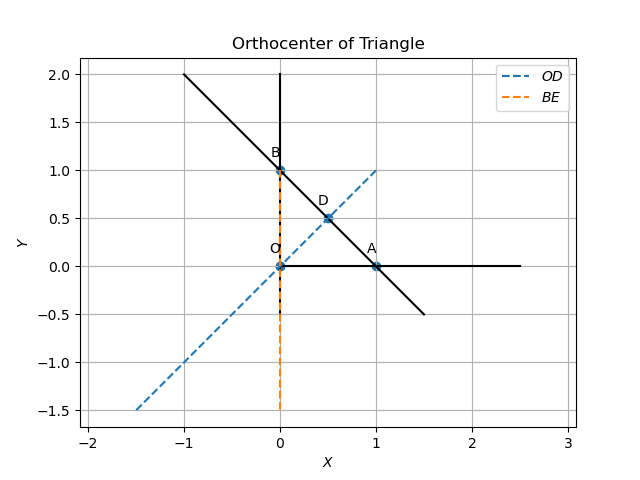
\includegraphics[scale=0.5]{fig1.png}
  \caption{$r_{1}=2,r_{2}=3$}
  \label{fig:circle assignment}
\end{figure}
\begin{figure}[h!]
  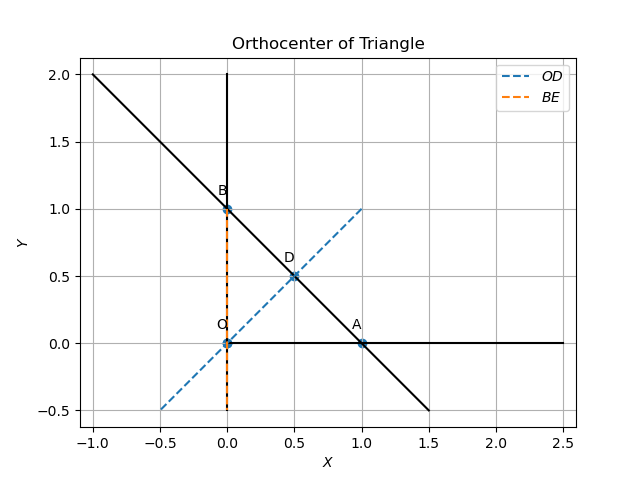
\includegraphics[scale=0.5]{fig2.png}
  \caption{$r_{1}=4,r_{2}=3$ }
  \label{fig:circle assignment}
\end{figure}
\begin{figure}[h!]
  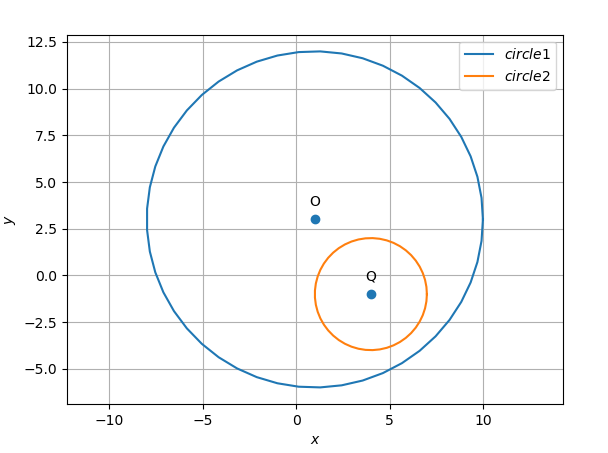
\includegraphics[scale=0.5]{fig3.png}
  \caption{$r_{1}=9,r_{2}=3$}
  \label{fig:circle assignment}
\end{figure}
\end{document}
